\documentclass[a4paper,norsk]{article}
\usepackage[latin1]{inputenc}
\usepackage[T1]{fontenc}
\usepackage{babel,textcomp,listings, subfigure,graphicx}
                                    
\title{Mandatory assignment 1, MEK4300}
\author{Sebastian Gjertsen}
\begin{document}
\maketitle
I have added all the python code with the email as .py files. 
\section*{i)}
In the first exercise we verified the analytical solutions of Poiseuille flow on three different geometries. Ellipse, eccentric annulus and equilateral triangle
\newline
First we look at Ellipse:
\newline
\begin{tabular}{l*{6}{c}r}
Mesh size              & CG & u-error & Q-error \\
\hline
0.349693241221 & 1 & 0.0175131635342 & 0.201811218507 \\
0.180720615753 & 1 & 0.033365539562 & 0.283682791213 \\
0.119623532036 & 1 & 0.0369504946463 & 0.298759959614\\
0.349693241221 & 2 & 0.0404398006589 & 0.309109678417 \\
0.180720615753& 2 & 0.0395051126483 & 0.312338039779 \\
0.119623532036 & 2 & 0.0393769579412 & 0.312804233035\\
\end{tabular}
\newline
Triangle:
\newline
\begin{tabular}{l*{6}{c}r}
Mesh size              & CG & u-error & Q-error \\
\hline
0.241111111111 & 1 & 1.20998709897 & 0.0250047363901\\
0.119935369941 & 1 & 1.20863104525 & 0.00748744892452\\
0.0744466995367 & 1 & 1.20886207311 & 0.00314150422326\\
0.241111111111 & 2 &  1.20888275059 & 3.08070312616e-05 \\
0.119935369941 & 2 & 1.20889036886 & 2.16354879279e-06 \\
0.0744466995367 & 2 & 1.20889077371 & 4.33605035322e-07 \\
\end{tabular}
\newline
Eccentric annulus:
\newline
\begin{tabular}{l*{6}{c}r}
Mesh size              & CG & Q-error \\
\hline
0.281069159834 & 1 & 4.52547426458 \\
0.199165514514 & 1 & 1.8915523401 \\
0.136943057055 & 1 & 0.957647075101\\
0.281069159834 & 2 & 3.38015721345\\
0.199165514514 & 2 & 1.36516979556\\
0.136943057055 & 2 & 0.664770215439\\
\end{tabular}
\newpage
\section*{ii)}
In part 2 we do not have an analytical solution, so i added a picture of the plot of F vs x. Where I have used CG 2 elements.
The first picture is for Newton:
\newline
\newline
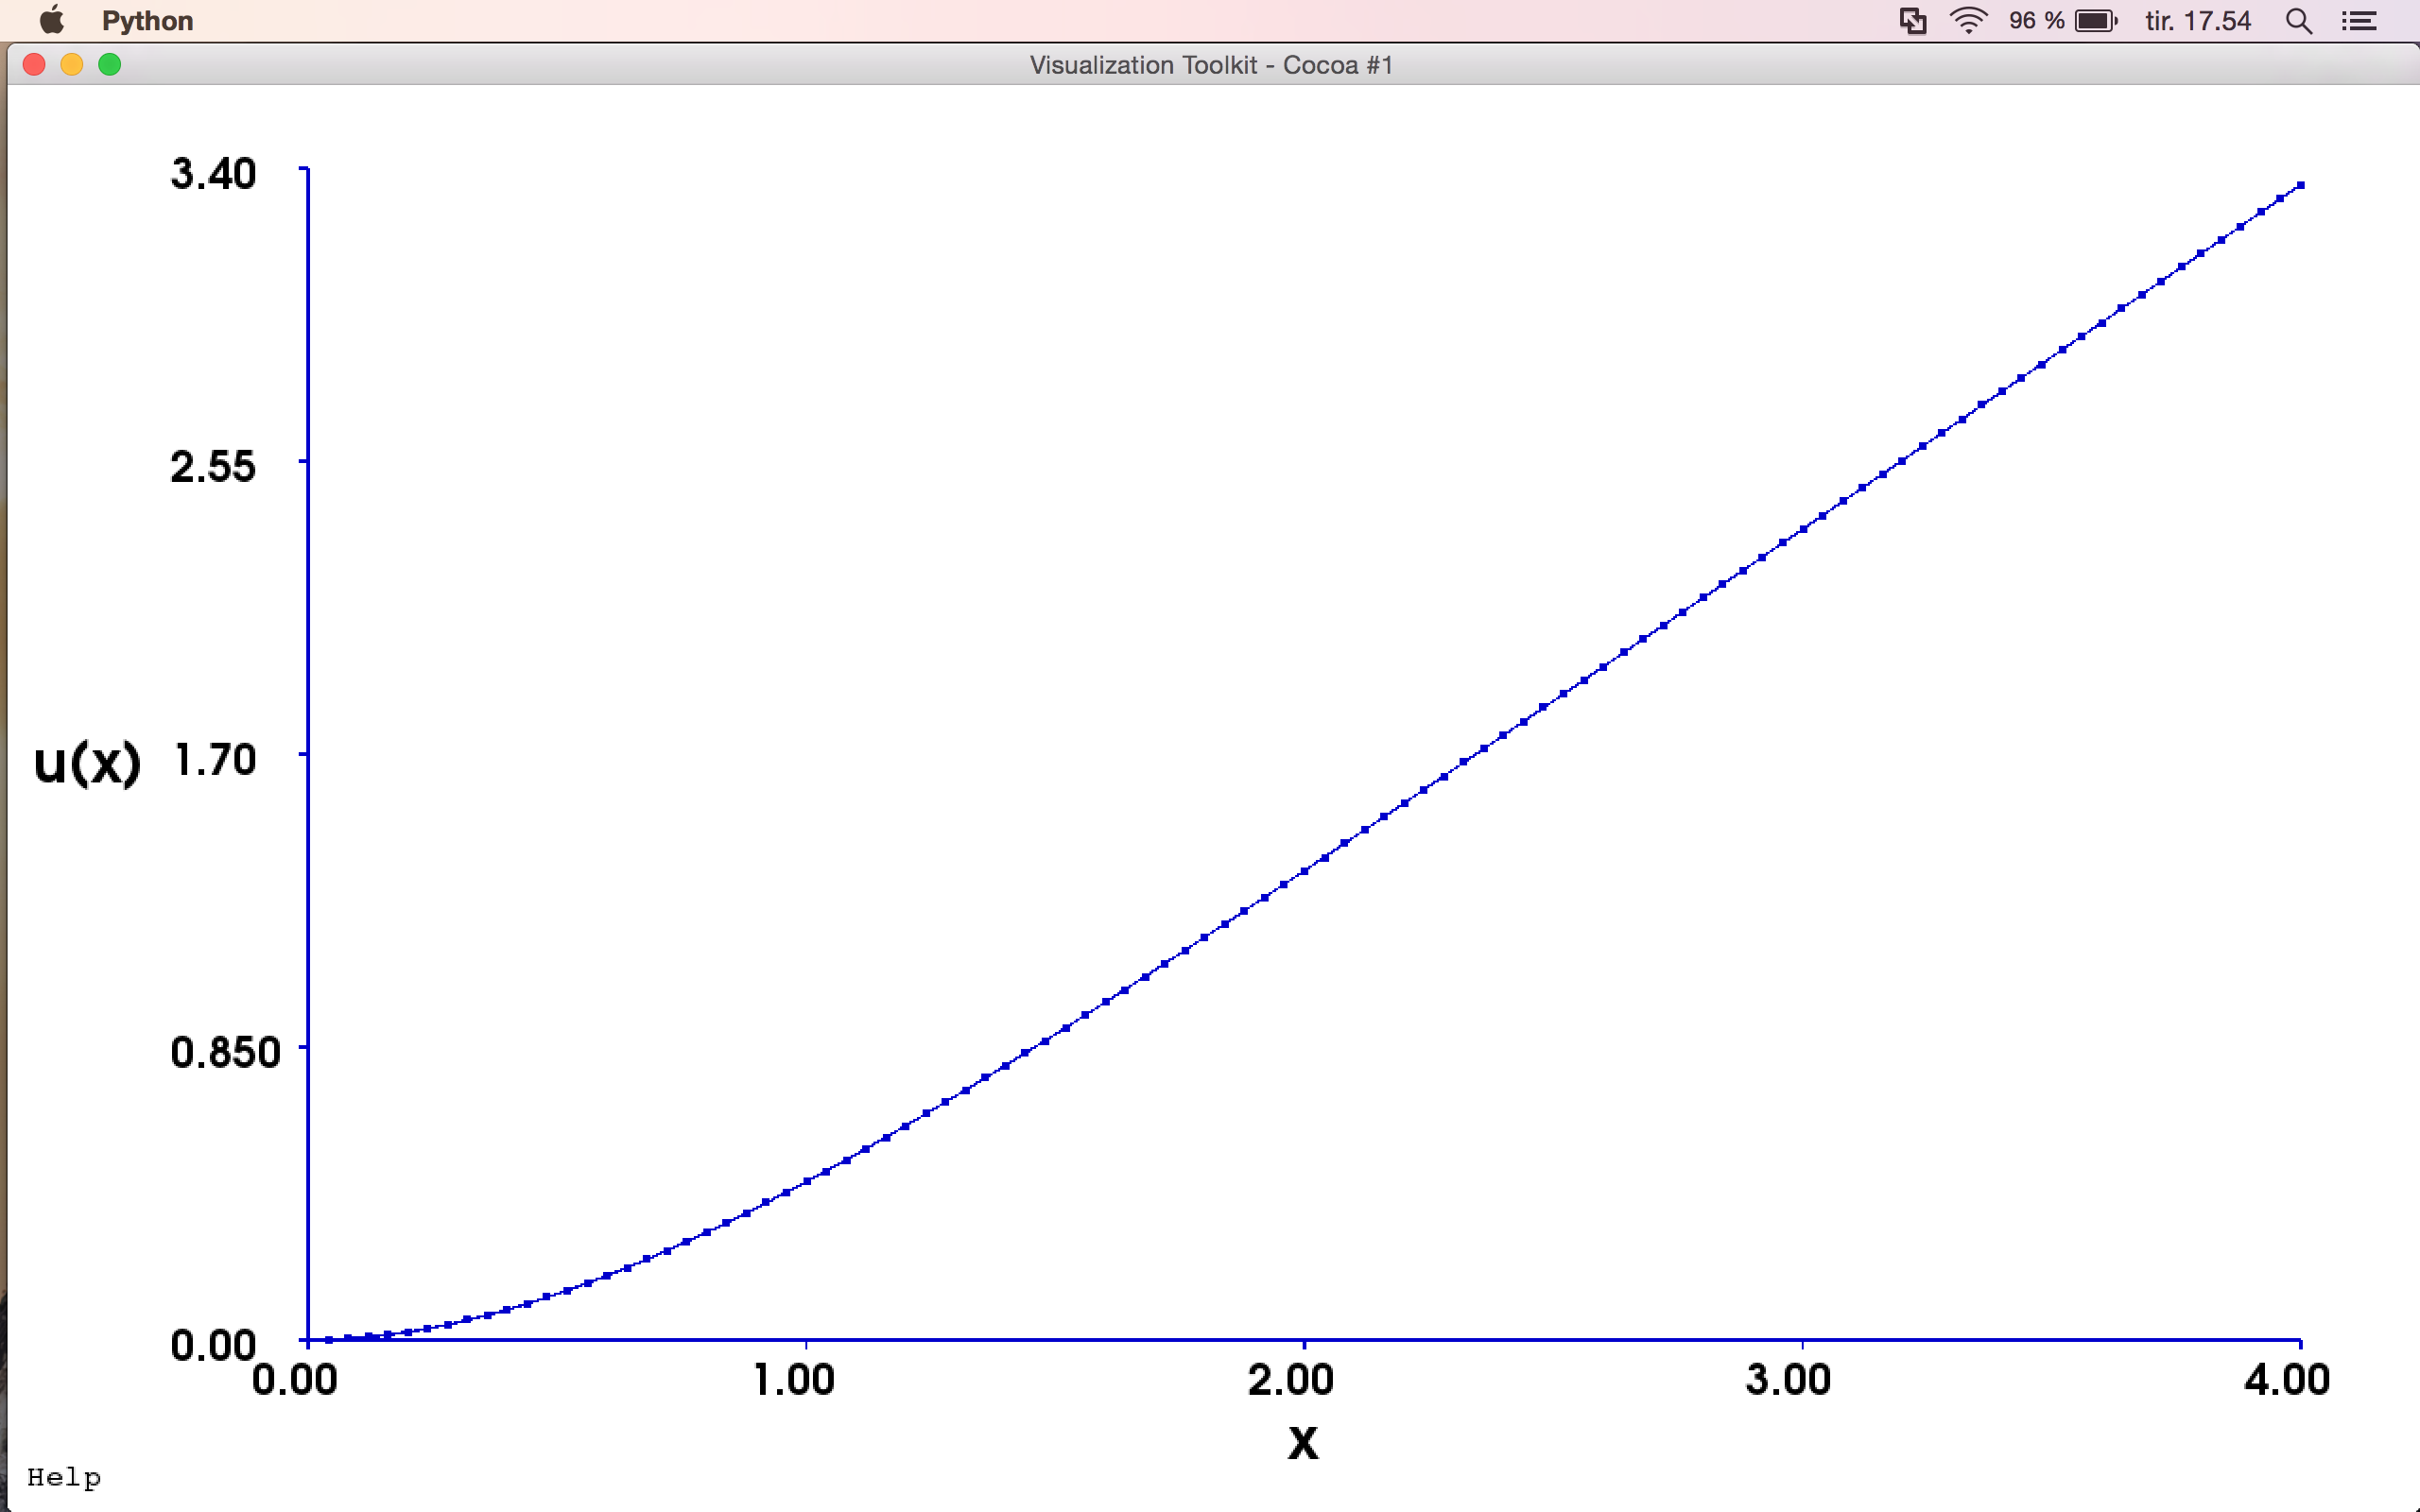
\includegraphics[trim = 5mm 0mm 2mm 25mm, clip, scale=0.3]{Newton_F.png}
\newline
\newline
Next is Picard:
\newline
\newline
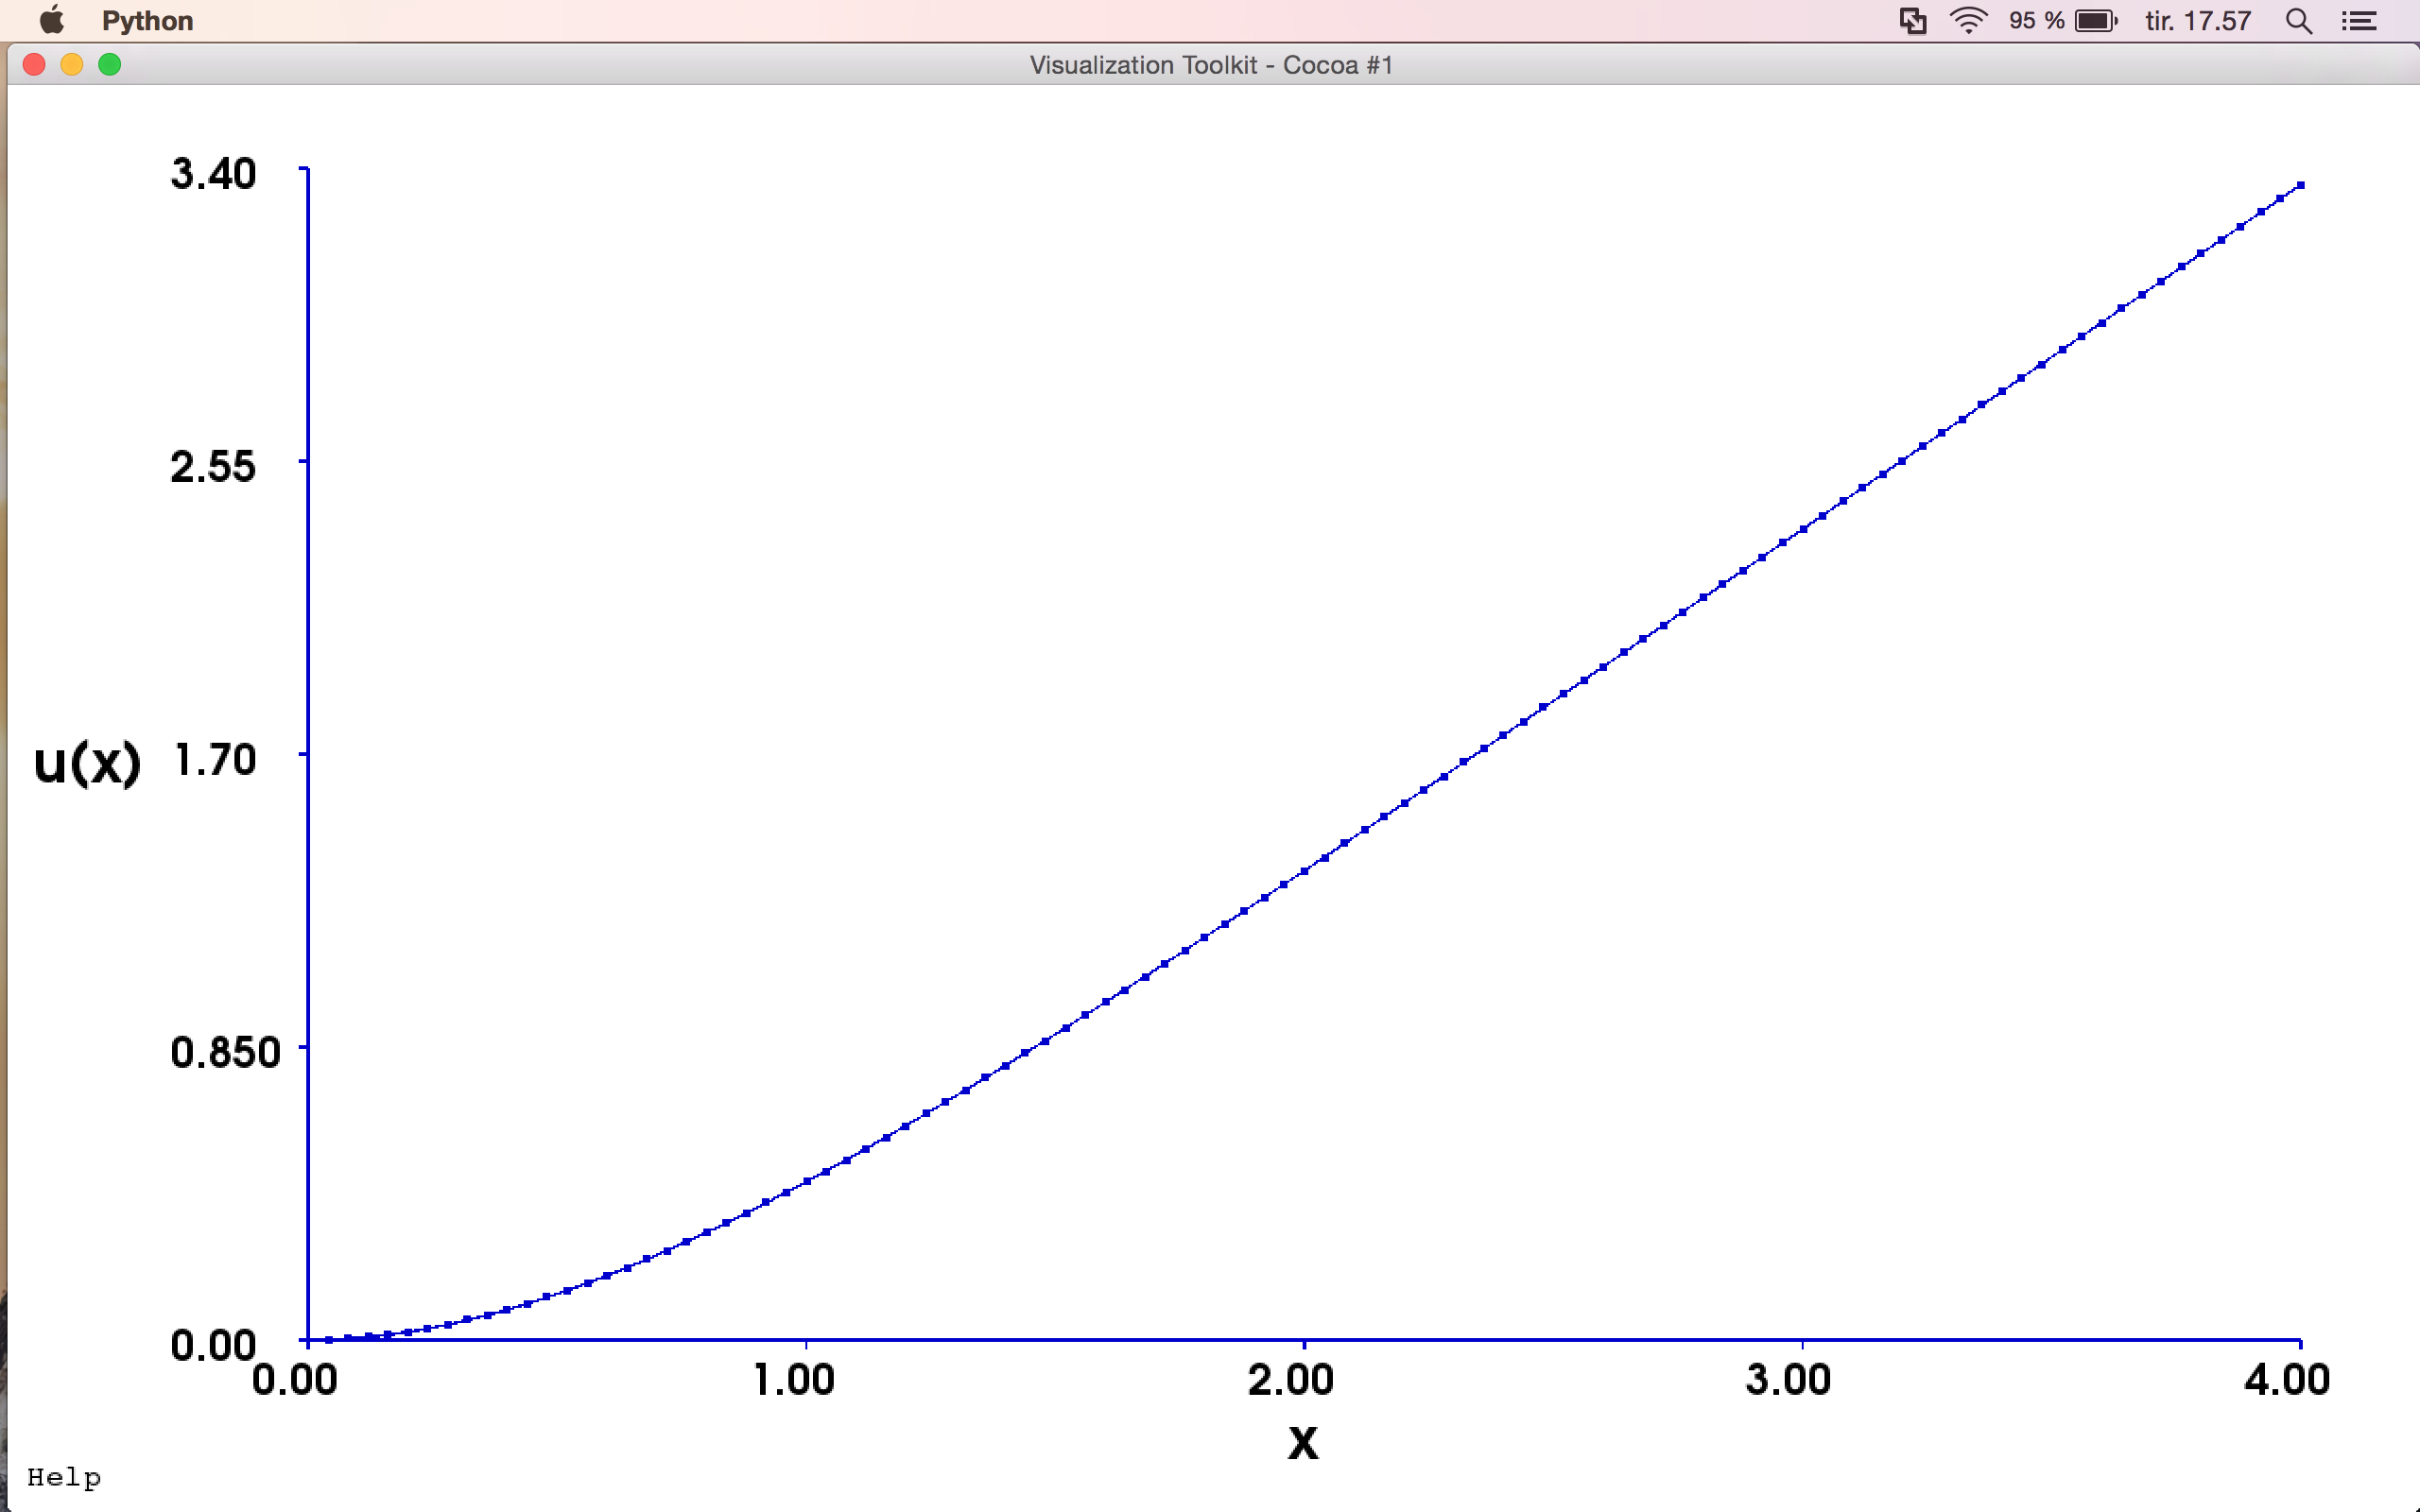
\includegraphics[trim = 5mm 0mm 0mm 25mm, clip, scale=0.3]{Picard_F.png} \newline
Since the two solutions look similar they seem to be correct.


\newpage
\section*{iii)}
In this exercise we were asked to compute the position of the central eddy, which is formed from stokes flow in a cavity driven square. I computed the streamfunction, and used its lowest value since the cavity had a positive(right) direction, to find the where the eddy had a center. 
\newline
The streamfunction plotted:

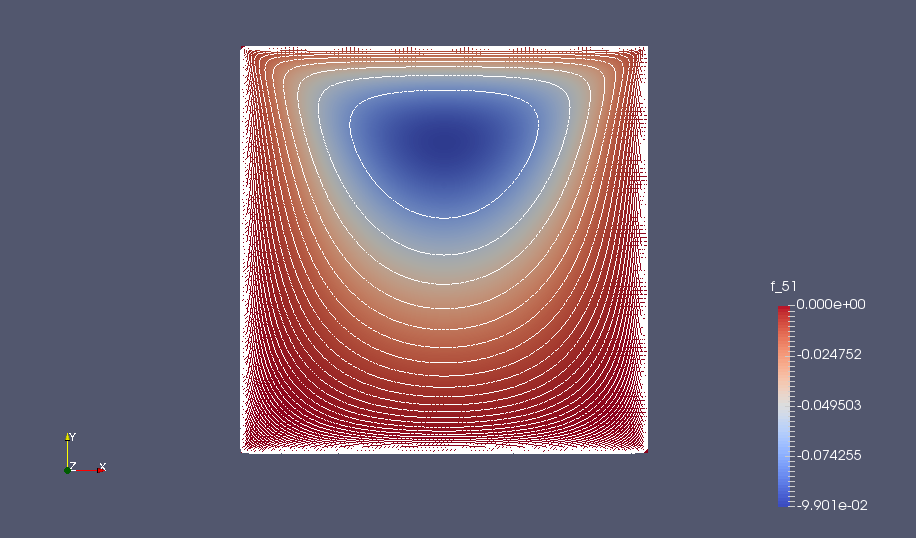
\includegraphics[trim = 0mm 0mm 0mm 0mm, clip, scale=0.4]{Cavity_psi.png}
\newline
\newline
I found the center eddys location to be (0.50,  0.76)
\newpage
\section*{iv)}
\subsection*{a)}
We were asked to make a rectangular mesh with a step. The length of the mesh was L and sides where 0.5L and the step was 0.1 L. I made the mesh so that origo was at the bottom of the mesh, in the middle, directly beneath the edge. I also made the mesh more fine at the step since there are more things happening here. \newline
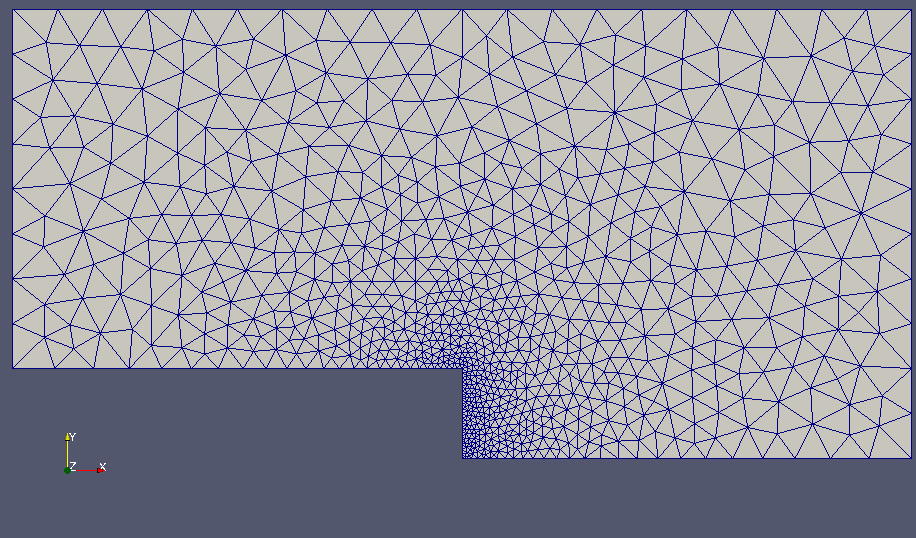
\includegraphics[trim = 0mm 0mm 0mm 0mm, clip, scale=0.4]{step_mesh.png}
\newline

In this exercise i did the same procedure as the iii), only now computing the streamfunction with weak boundary condtions instead of Dirichlet. 
I found the position of the main eddy with three different meshes: \newline
\newline
\begin{tabular}{l*{6}{c}r}
   Vertices & Cells & Center eddy\\
 \hline 
79 &127 & (-0.5000, 0.1000) \\
4790 & 9305& (-0.4614, 0.1000 )\\
18731 & 36914 & (0.0353, 0.0392)\\ 
74127 & 147160 & (0.0351, 0.0392) \\
\hline
\end{tabular}
\newline
\newline
Where the two last seem most logical taken the mesh in consideration.
\newline
\subsection*{b)}
Here are two picture of the streamfunction over the step in both positive and negative direction:
\newline
\newline
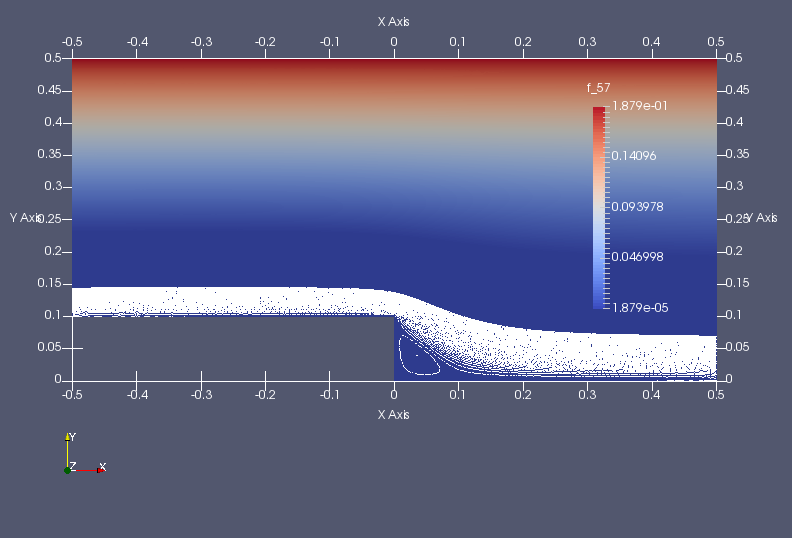
\includegraphics[trim = 0mm 0mm 0mm 0mm, clip, scale=0.4]{Stream_down.png}
\newline
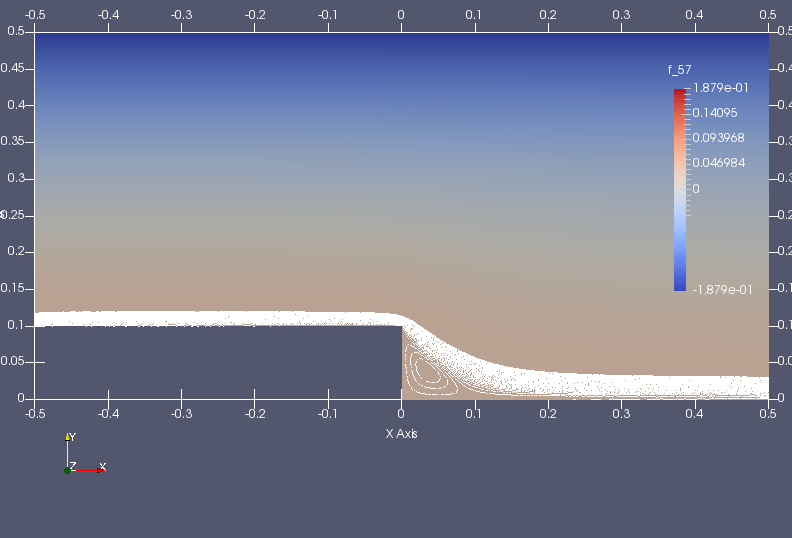
\includegraphics[trim = 0mm 0mm 0mm 0mm, clip, scale=0.4]{Stream_up.png}

\subsection*{c)}
In this section I calculated the flux going in and out of the left and right side of the boundary. And got: \newline
Flux left:  -0.212606783972 \newline
Flux right:  0.212605013813 \newline
\newline
Since these numbers are almost identical and with opposite signs, we can say mass is being conserved.

\subsection*{d)}
If we reverse the direction we can see from the pictures that the vortex stays in the same spot. This is because the step is geometrically the only thing causing a vortex regardless of direction. The step is causing a change in velocity and pressure, giving the fluid rotation.

\subsection*{e)}
In this section we calculated the normal stress on the "floor". And could see when we sent the flow down the step that we have a stress going down in the "floor" and the opposite happening when we sent the flow up the stairs. This coincides with what we observe with airplanes getting positive force to fly.
\newline
In positive direction: \newline
Normal stress:  121.504028211 \newline
In negative direction : \newline
Normal stress:  -121.504028211

























\end{document}